\documentclass[border=15pt]{standalone}
\usepackage{amsmath,amssymb,mathtools}
\usepackage{tikz}
\usepackage{pgfplots}
\usepackage{pgf}
\begin{document}
	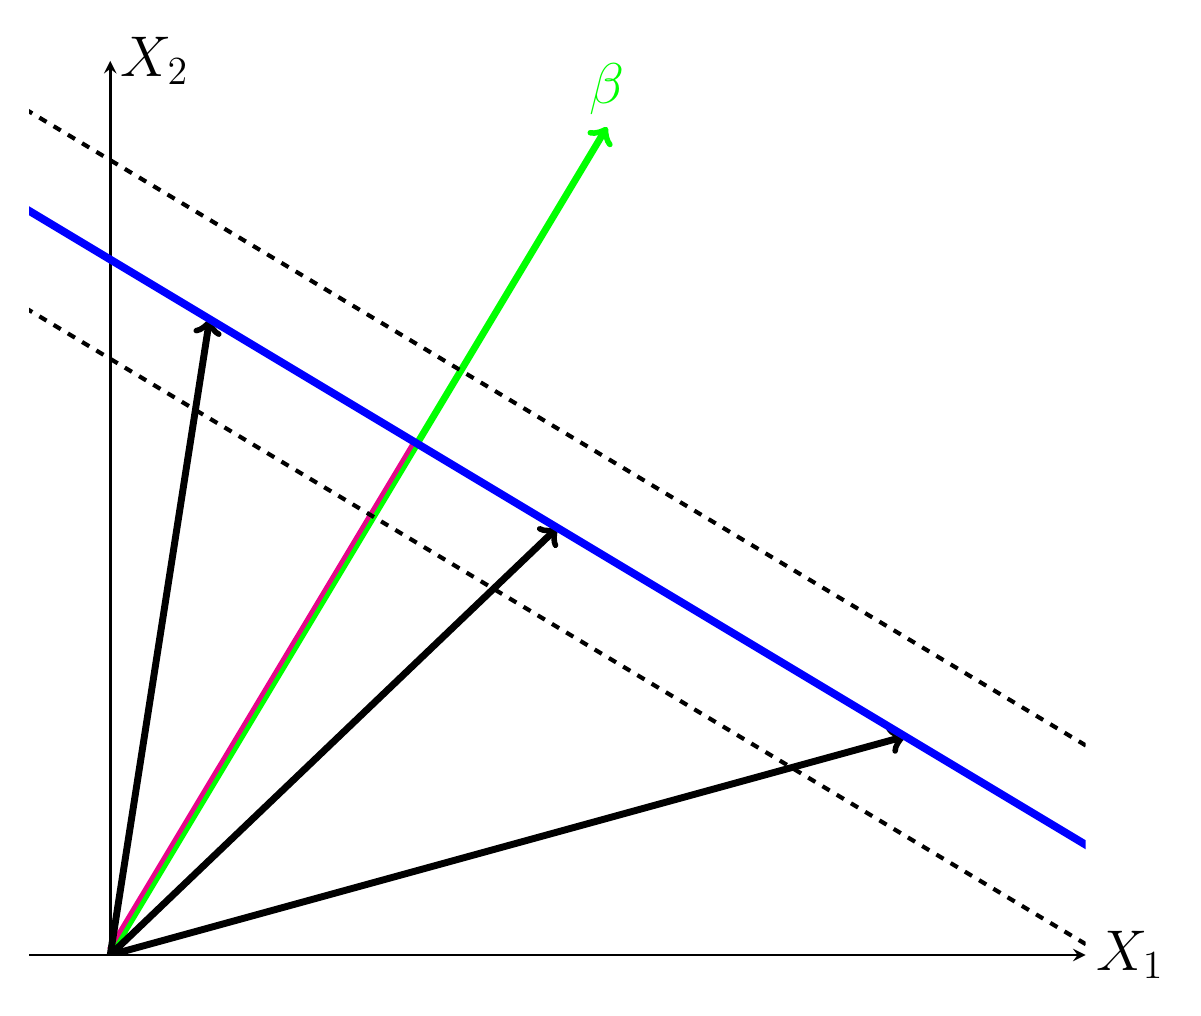
\begin{tikzpicture}
		\begin{axis}[
			xmin=0,
			xmax=9,
			ymin=0,
			ymax=9,
			axis equal,
			width=15cm,
			axis x line=center,
			axis y line=center,
			xmajorticks=false,
			ymajorticks=false,
			ylabel style={right,font=\huge},
			ylabel=$X_2$,
			xlabel style={above,right,font=\huge},
			xlabel=$X_1$,
			line width=1pt
			]
			%\addplot[no markers, domain=-1:11]{(5/3)*x};
			\draw[magenta,line width=2.5pt] (axis cs:0,0.05)--(axis cs:3.078235,5.177058);
			\draw[->,green,line width=2.5pt] (axis cs:0,0)--(axis cs:5,8.333) node[above,pos=1,font=\huge]{\textcolor{green}{$\mathbf{\beta}$}};
				\draw[magenta,thick] (axis cs:0,0.05)--(axis cs:3.078235,5.177058);
			\draw[->,line width=2.5pt] (axis cs:0,0)--(axis cs:8,2.2);
			\draw[->,line width=2.5pt] (axis cs:0,0)--(axis cs:4.5,4.3);
			\draw[->,line width=2.5pt] (axis cs:0,0)--(axis cs:1,6.4);
			
			\addplot[no markers,domain=-1:11,line width=2.8pt,blue]{-0.6*x+7};
			\addplot[no markers, domain=-1:11,line width=1.5pt,dashed]{-0.6*x+8};
			\addplot[no markers, domain=-1:11,line width =1.5pt,dashed]{-0.6*x+6};
		\end{axis}
	\end{tikzpicture}

\end{document}